\documentclass[a4paper]{article}

%% Language and font encodings
\usepackage[english]{babel}
\usepackage[utf8]{inputenc}

% Set page size and margins
\usepackage[a4paper,top=2cm,bottom=2cm,left=2.5cm,right=2.5cm,marginparwidth=1.75cm]{geometry}

%----------- APA style references & citations (starting) ---
% Useful packages
%\usepackage[natbibapa]{apacite} % APA-style citations.

\usepackage[style=apa, backend=biber]{biblatex} % APA 7th edition style citations using biblatex
\addbibresource{references.bib} % Your .bib file

% Formatting DOI in APA-7 style
%\renewcommand{\doiprefix}{https://doi.org/}

% Add additional APA 7th edition requirements
\DeclareLanguageMapping{british}{british-apa} % Set language mapping
\DeclareFieldFormat[article]{volume}{\apanum{#1}} % Format volume number

% Modify 'and' to '&' in the bibliography
\renewcommand*{\finalnamedelim}{%
  \ifnumgreater{\value{liststop}}{2}{\finalandcomma}{}%
  \addspace\&\space}
  
%----------- APA style references & citations (ending) ---


\usepackage{amsmath}
\usepackage{graphicx}
\usepackage[colorlinks=true, allcolors=blue]{hyperref}
\usepackage{hyperref}
\usepackage{orcidlink}
\usepackage[title]{appendix}
\usepackage{mathrsfs}
\usepackage{amsfonts}
\usepackage{booktabs} % For \toprule, \midrule, \botrule
\usepackage{caption}  % For \caption
\usepackage{threeparttable} % For table footnotes
\usepackage{algorithm}
\usepackage{algorithmicx}
\usepackage{algpseudocode}
\usepackage{listings}
\usepackage{enumitem}
\usepackage{chngcntr}
\usepackage{booktabs}
\usepackage{lipsum}
\usepackage{subcaption}
\usepackage{authblk}
% \usepackage[T1]{fontenc}    % Font encoding
\usepackage{csquotes}       % Include csquotes
\usepackage{diagbox}


% Customize line spacing
\usepackage{setspace}
\onehalfspacing % 1.5 line spacing

% Redefine section and subsection numbering format
\usepackage{titlesec}
\titleformat{\section} % Redefine section numbering format
  {\normalfont\Large\bfseries}{\thesection.}{1em}{}

% Define a new command for the fourth-level title.
\newcommand{\subsubsubsection}[1]{%
  \vspace{\baselineskip}% Add some space
  \noindent\textbf{#1\\}\quad% Adjust formatting as needed
}
% Change the position of the table caption above the table
\usepackage{float}   % for customizing caption position
\usepackage{caption} % for customizing caption format
\captionsetup[table]{position=top} % caption position for tables

% Define the unnumbered list
\makeatletter
\newenvironment{unlist}{%
  \begin{list}{}{%
    \setlength{\labelwidth}{0pt}%
    \setlength{\labelsep}{0pt}%
    \setlength{\leftmargin}{2em}%
    \setlength{\itemindent}{-2em}%
    \setlength{\topsep}{\medskipamount}%
    \setlength{\itemsep}{3pt}%
  }%
}{%
  \end{list}%
}
\makeatother

% Suppress the warning about \@parboxrestore
\pdfsuppresswarningpagegroup=1


%-------------------------------------------
% Paper Head
%-------------------------------------------
\title{A replication study of transformer-based TabPFN for assessing the applicability of neural-network based solutions in tabular classification.}

\author[1]{Kartikey Chauhan}
\affil[1]{\small Data Science \& Analytics, Toronto Metropolitan University}

\date{}  % Remove date

\begin{document}
\maketitle

\begin{abstract}
We perform a replication study of TabPFN, a transformer-based model for tabular data classification. We evaluate the model on a set of benchmark datasets and compare its performance against traditional machine learning methods and state-of-the-art AutoML systems. Our results show that TabPFN outperforms the baselines on most datasets, demonstrating the potential of neural-network based solutions in tabular classification tasks. We also provide an empirical review of TabPFN's claims and discuss potential avenues for further scaling and modifications based on the latest advancements in the Transformer space.

\end{abstract}

\textbf{Keywords}: TabPFN, Transformers, Tabular Data, Classification, Machine Learning

%-------------------------------------------
% Paper Body
%-------------------------------------------
%--- Section ---%
\section{Introduction}

Deep Learning has revolutionized the field of AI and led to remarkable achievements in applications involving image and text data. In particular, large transformer-based models trained on massive corpora, are disrupting machine learning in many areas. However, when it comes to tabular (a.k.a. structured) data, traditional machine learning methods, such as gradient-boosted decision trees have shown superior performance over deep learning. 

Recently, TabPFN \cite{hollmann2023tabpfn} \footnote{\url{https://github.com/automl/TabPFN}} proposes a radical change to how tabular classification is done, introducing a pre-trained Transformer that is able to perform classification without training. This project aims to replicate and do an empirical review of TabPFN's claims, while potentially exploring avenues for further scaling and modifications based on latest advancements in the Transformer space.

%--- Section ---%
\section{Background on TabPFN}\label{sec2}

\begin{figure}[!ht]
  \centering
  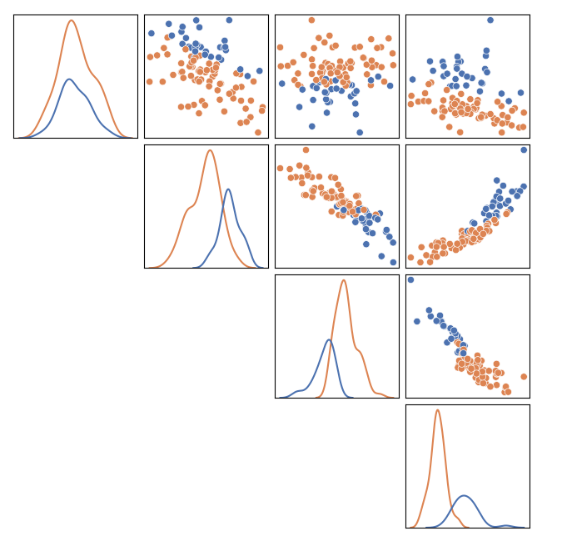
\includegraphics[width=0.4\linewidth]{figures/priors_visualized.png}
  \caption{\label{fig:priors} Visualization of Prior samples.}
  \end{figure}

\subsection{TabPFN Architecture}\label{subsec1}

TabPFN proposed a two-stage approach for tabular data classification:
\begin{itemize}
  \item First, meta-learn to approximate Bayesian inference using synthetic datasets.
  \item Second, use the labeled samples \textit{in context} to classify unlabelled samples.
\end{itemize}

TabPFN is trained on a large number of synthetic datasets generated from a carefully designed prior distribution. This prior incorporates principles from causal reasoning and a preference for simple structures. Here are some key details about the prior used in TabPFN:

\begin{enumerate}
  \item \textbf{Structural Causal Models (SCMs)}: The prior entails a space of structural causal models, which are used to generate the synthetic datasets. This allows TabPFN to learn the causal relationships and structures present in tabular data.
  
  \item \textbf{Preference for Simplicity}: The prior has a preference for simpler causal structures over more complex ones. This bias towards simplicity helps TabPFN avoid overfitting and generalize better to new datasets.
  
  \item \textbf{Bayesian Neural Networks (BNNs)}: In addition to SCMs, the prior also includes Bayesian neural networks as a possible data generating mechanism. This allows TabPFN to capture non-linear relationships in the data.
  
  \item \textbf{Varying Dataset Characteristics}: The synthetic datasets are generated with varying numbers of features (up to 100), classes (up to 10), and sample sizes (up to 1024). This exposure to diverse dataset characteristics during training helps TabPFN generalize to a wide range of tabular problems.
  
  \item \textbf{Hyperparameter Sampling}: The prior also includes sampling of various hyperparameters, such as MLP weight dropout, input feature scaling, and whether to sample the target variable from the last MLP layer or not.
\end{enumerate}

By training on this carefully designed prior distribution, TabPFN learns to approximate Bayesian inference on tabular data tasks, allowing it to quickly adapt to new datasets through in-context learning without additional training or hyperparameter tuning.


% Code block 
\begin{verbatim}
  TransformerModel(
    (transformer_encoder): TransformerEncoderDiffInit(
      (layers): ModuleList(
        (0-11): 12 x TransformerEncoderLayer(
          (self_attn): MultiheadAttention(
            (out_proj): NonDynamicallyQuantizableLinear(in_features=512, out_features=512, bias=True)
          )
          (linear1): Linear(in_features=512, out_features=1024, bias=True)
          (dropout): Dropout(p=0.0, inplace=False)
          (linear2): Linear(in_features=1024, out_features=512, bias=True)
          (norm1): LayerNorm((512,), eps=1e-05, elementwise_affine=True)
          (norm2): LayerNorm((512,), eps=1e-05, elementwise_affine=True)(dropout1): Dropout(p=0.0, inplace=False)
          (dropout2): Dropout(p=0.0, inplace=False)
        )
      )
    )
    (encoder): Linear(in_features=100, out_features=512, bias=True)
    (y_encoder): Linear(in_features=1, out_features=512, bias=True)
    (decoder): Sequential(
      (0): Linear(in_features=512, out_features=1024, bias=True)
      (1): GELU(approximate='none')
      (2): Linear(in_features=1024, out_features=10, bias=True)
    )
    (criterion): CrossEntropyLoss()
  )
  \end{verbatim}

%--- Insert an image comparing 4 classifiers ---%
\begin{figure}[!ht]
  \centering
  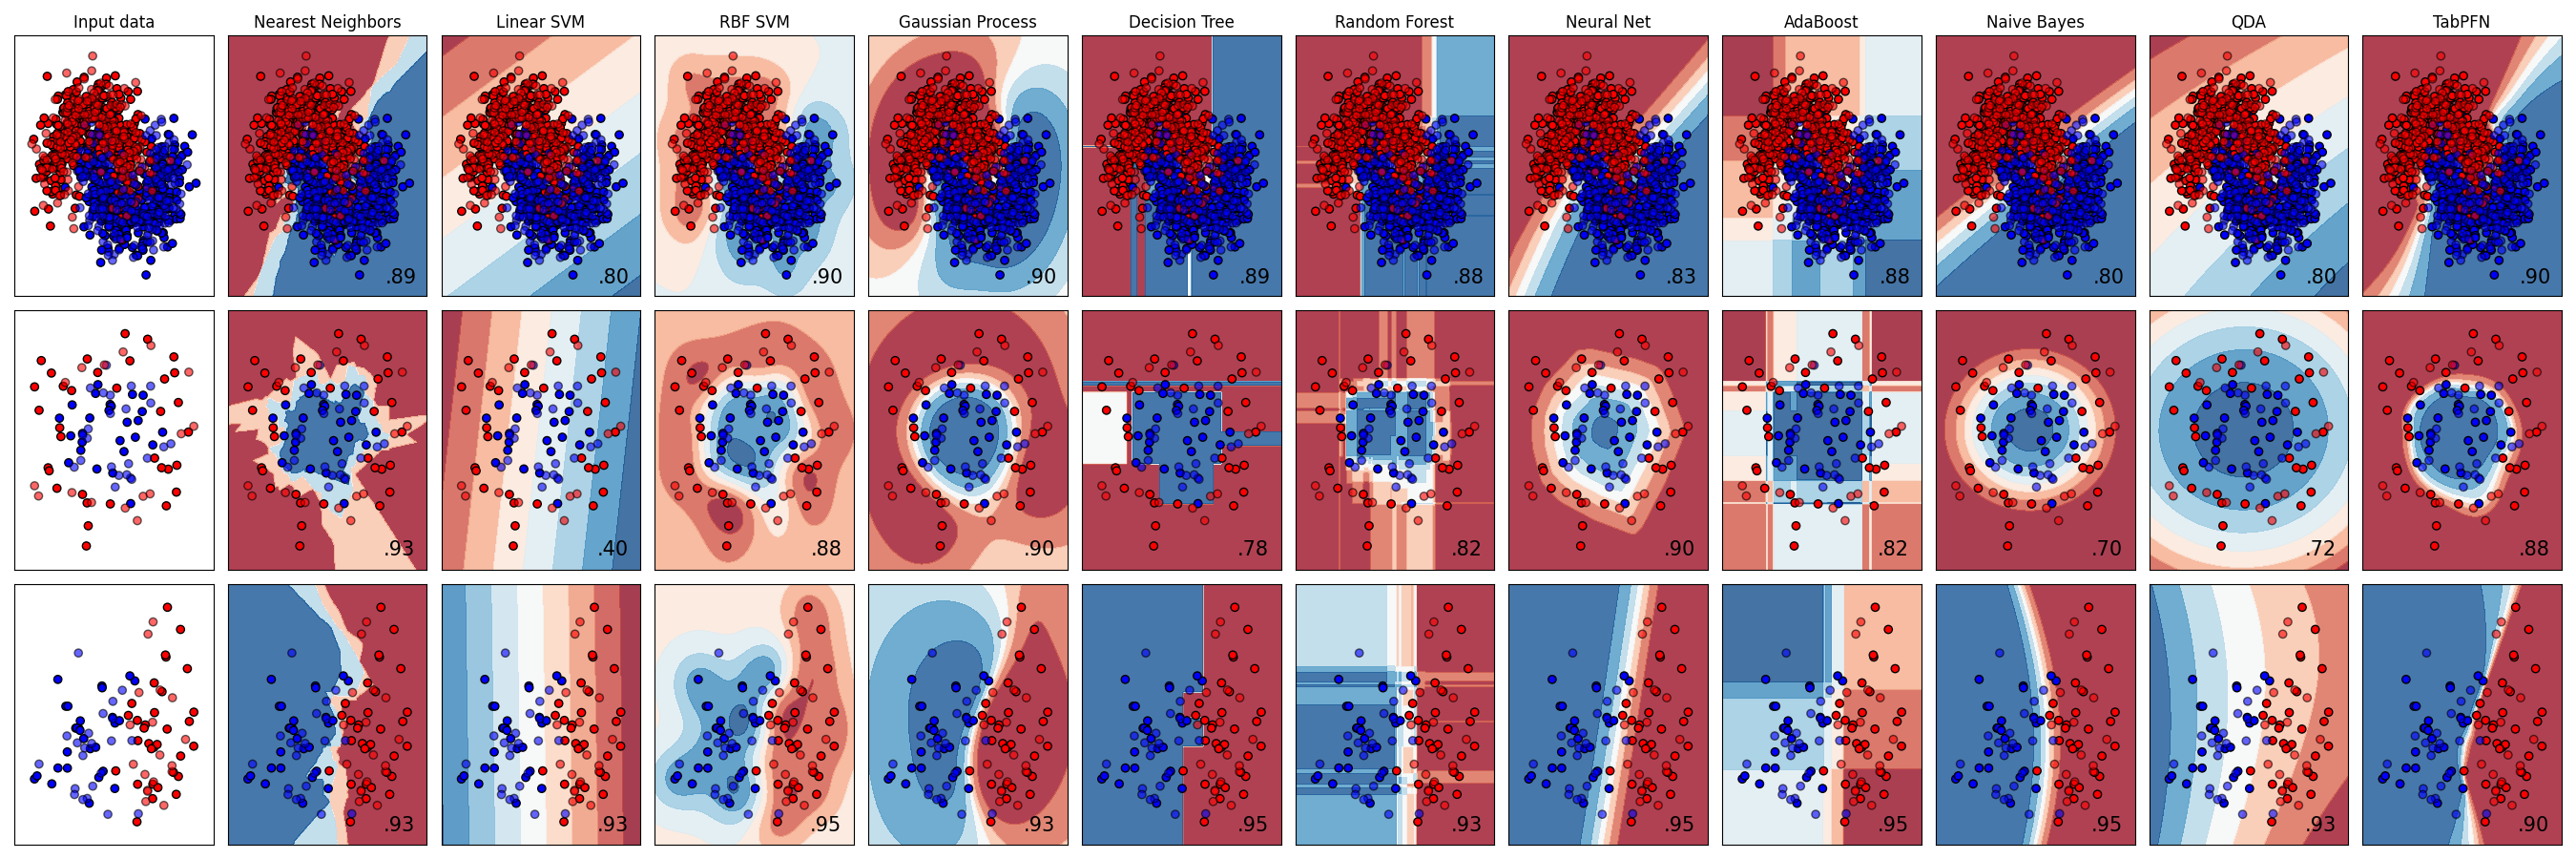
\includegraphics[width=0.8\linewidth]{figures/classifier_decision_boundary.png}
  \caption{\label{fig:classifier_decision_boundary} Decision boundaries on toy datasets generated with scikit-learn}
  \end{figure}
  
% 
\subsection{How to create sections and subsections}
Simply use the section and subsection commands, as in this example document! With Overleaf, all the formatting and numbering is handled automatically according to the template you've chosen. If you're using the Visual Editor, you can also create new sections and subsections via the buttons in the editor toolbar.

\subsection{This is an example for second level head - subsection head}\label{subsec1}
\lipsum[5]

\subsubsection{This is an example for third level head - subsubsection head}\label{subsubsec1}
\lipsum[6]

\subsubsubsection{This is an example for fourth level head - paragraph head}
\lipsum[7]


%--- Section ---%
\section{Replication and Evaluation}\label{sec3}

\subsection{Baselines}\label{subsec2}

We start with evaluation of the existing model provided the authors of TabPFN.  We compare against five standard ML methods and two state-of-the-art AutoML systems for tabular data.

\subsubsection{Datasets}\label{subsubsec2}
\lipsum[8]

\subsubsubsection{This is an example for fourth level head - paragraph head}
\lipsum[9]


%--- Section ---%
\section{Conclusions}
Some conclusions here.

%-------------------------------------------
% References
%-------------------------------------------

% Print bibliography
\printbibliography




%-------------------------------------------
% Appendix
%-------------------------------------------
% Activate the appendix in the doc
% from here on sections are numerated with capital letters 
%\appendix

% Change equation numbering format to be sequential within sections in the appendix
\renewcommand\theequation{\Alph{section}\arabic{equation}} % Redefine equation numbering format
\counterwithin*{equation}{section} % Number equations within sections
\renewcommand\thefigure{\Alph{section}\arabic{figure}} % Redefine equation numbering format
\counterwithin*{figure}{section} % Number equations within sections
\renewcommand\thetable{\Alph{section}\arabic{table}} % Redefine equation numbering format
\counterwithin*{table}{section} % Number equations within sections

\begin{appendices}

%--- Section ---%
\section{Some Notation}
\lipsum[10]

\subsection{Appendix subsection title here}
\lipsum[14]

\end{appendices}


\end{document}